\section{Approach}
\label{sec:method}

In this section, we describe our proposed approach which shown in 
Figure ~\ref{fig:workflow}.
%As can be seen from Figure ~\ref{fig:workflow}, our recommender system 
%uses three dataset: 
%1) the change history, 2) the class dependency  
%and 3) the test cases. 
There are two major activity in our proposed approach: 
Fault severity measurement and cost aware test case prioritization. 
Below we describe each activity in detail. 

\begin{figure*}[!hb]
	\centering
	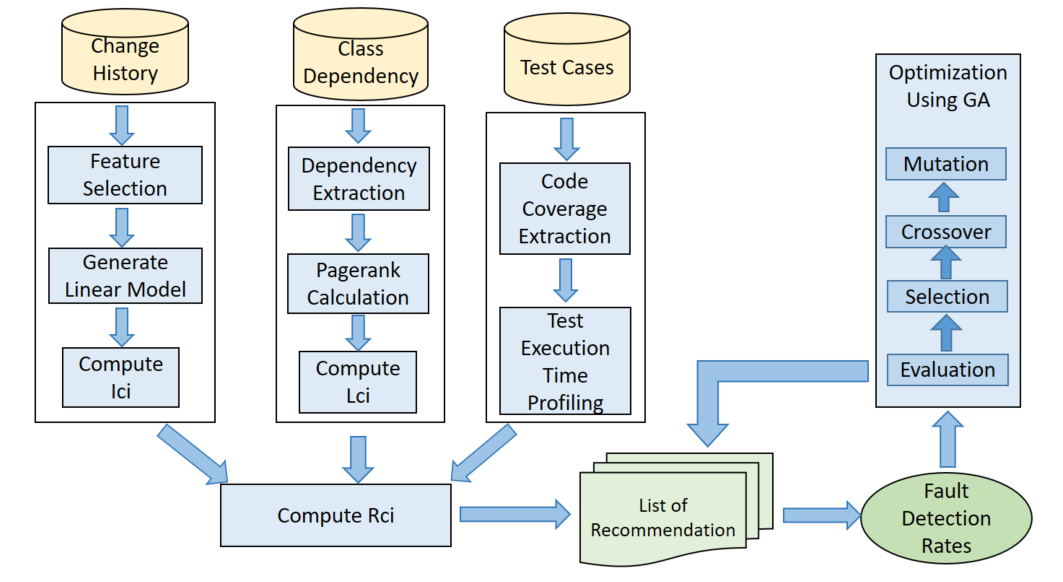
\includegraphics[width=0.75\linewidth]{./workflow4.png}
	\vspace*{3pt}
	\caption{An Overview of the Proposed Technique}
	\label{fig:workflow}
\end{figure*} 

%\subsection{Context-aware Recommender System}
\subsection{Fault Severity Measurement}
%Recommender system have been used in different areas as a powerful and popular tool 
%to ease the decision making process for users based on two main inputs;
%users rating and items characteristics. 
%Like other areas, recommender system have been used
%in software engineering domain for variety of purposes.
%A typical scenario of test case prioritization for regression testing is retesting the entire system 
%from most important test cases until we find all faults. 
%To do this one of the most commonly used techniques is
%greedy technique; which prioritized test cases based on their code coverage. 
%Although, greedy technique is powerful but it does not utilize other source code information 
%that might be a potential key for finding the most critical part of the system that
%their risk of failure is higher than other parts. 
%In another word, we can apply several information other than code coverage to extract 
%hidden relation between the source code and the fault risk. 




% paraphe bala bere be study ya disscussion!!!!!!!!!!!!!!
The goal of our recommender system is to find a sorted list of test cases 
to balance above mentioned datasets. 
To implement this approach we proposed a cost-effective recommender system that uses three
datasets as input parameters for producing the list of most risky classes with considering 
their test cost. 
Traditionally, recommender systems use two main inputs for 
producing a ranking score for a specific item by the below formula:
  
\[
{R : User * Item }
\] 
 
Those recommender systems show a significant effect and  
provide the most related list but still they ignore the importance 
of contextual information. 
Our recommender system takes fault severity and test cost as the
input parameters for generating the
list of most important test cases that should be tested first. 


There are different ways to measure fault severity such as its fixing cost and 
the require time to find fault location, but
here we define bug severity as a combination
of the impact that a bug may induce on the system and the location of the bug. 
We defined our ranking formula as:

\[
{R : I_{Ci} * L_{Ci} * T_{Ci} }
\] 

where $I_{Ci}$ is the $change impact score$, $L_{Ci}$ is the 
score of location criticality and $T_{Ci}$ is the test case cost for testing class $C_{i}$. 
% here use jeff paper why the location matters? 
% later in subsection we will tlk about benefist of pagerank and location aware
In the following subsections, we explain the steps of calculating each parameter 
in detail. 

\subsubsection{Change History Analysis}

% the linear model calculates the change impact score!
The first phase of our proposed approach is change history
analysis. Change history has a significant role in the error proneness of code, 
according to the previous studies []. 
Although other code attributes such as statistic code metrics also might 
have an impact on faulty code or failure risk, we decided to choose
change history to avoid over-fitting. 
The process of change impact analysis has three major steps itself. 
First of all, we collected all change information and bug reports from the 
entire repository for each application. 
After collecting all change history information we applied feature selection
technique to find the most effective metrics that are likely causes of system failure. 
To select the most effective features we measured gain ratio for all features. 
In next phase, to evaluate the impact that a particular change may 
impose to the system, we generated a linear model from a set of collected 
change metrics and fault history. We also evaluated the accuracy of our linear model. 
	
	
	In order to evaluate the accuracy of our classification model, we used 
	10-fold cross validation and we repeated this process for several times. 
	Also, we used common accuracy indicator to determine the accuracy of 
	our model. Below Table ~\ref{tab:ConfusionMatrix} shows the confusion matrix that we used
	for accuracy evaluation. PC indicates the percentage of correctly classified 
	instances, TP indicates the number of classes that contains a bug and our classification
	model also classified them as a buggy classes, and FP is the number of classes that 
	are classified as buggy but they are clean. 
	
	
	\begin{table}[!ht]
		\caption{Confusion Matrix}
		\vspace*{-10pt}
		\begin{center}
			\begin{tabular}{|l||c||c||c|}
				\hline
				Metrics     & Predicted: No & Predicted: Yes &  \\ \hline
				Actual: No  &     TN = 33   &     FP =  63   & 96 \\ \hline
				Actual: Yes &     FN = 54   &     TP =  46   & 100 \\ \hline
				            &      87       &       109      & 196 \\ \hline
			\end{tabular}
			\end {center}
			\label{tab:ConfusionMatrix}
			\vspace*{-5pt}
	\end{table}
	
	A higher PC value means that our classifier model is efficient. 
	If PC is high, but the recall (TP) low, this means that our classifier classified a large number of
	classes as clean when they are not; this means that we missed many buggy classes during this phase
	for testing. However, if FP is high it means that our model detected many files as buggy when they 
	are clean and this will add extra cost for testing the system when it is not needed. 
	
	Finally, output of this part of our recommender system is $I_{Ci}$, which is a
	numerical value that indicates the impact of the change on a specific class.  
	
	
	
	%In section ~\ref{label}
	%we will explain the details of data collection and generating our linear model in details. 
	
	
	
	
	
	%assessing classification accuracy --> this is how we evaluate our classification
	% A Comparative Analysis of the Efficiency of Change Metrics and Static Code Attributes for Defect Prediction
	
	
	%!!!!!!!!!!!!!!!!!!!!!!!!!!!!!!!!!!!!!!
	
	
	%	A common strategy for training reliable and stable classification
	%	(or regression) models when only one data set for both model
	%	training and testing is available is as follows: we repeat several
	%	times 10-fold cross-validation for computing various error
	%	measures [28]. For each 10-fold cross-validation we calculate the
	%	following accuracy indicators: percentage of correctly classified
	%	instances, PC, the true positive rate, TP, and the false positive
	%	rate, FP. We explain the meaning of those indexes with a simple
	%	example: let us assume that for a particular data set, containing
	%	105 instances (files in our case), a model provides the following
	%	predictions: 43 files are defect free and 62 defective. However, in
	%	reality 32 files are defect free and 73 have at least one defect.
	%	Knowing the true class distribution (i.e., if a file is defect free or
	%	not) we can summarize our prediction results using the so-called
	%	confusion matrix (see Table 1).
	
	
		
%		1 means that a file has one or more defects while 0 means that it is
%		defect free. The meaning of the entries of the confusion matrix is
%		self-explanatory: the value in the gray shadowed cell for example
%		tells us that our model predicts 23 files as defect free, which in
%		reality have at least one defect! This is for sure not what we want
%		as detecting and fixing errors in later phases of development or
%		after the software has been deployed at a customer’s site can be
%		very costly. We rather prefer that our model predicts that a file
%		has a defect, but in reality doesn’t (our model predicts 12 such
%		files). In this case we waste resources for inspecting the file but in
%		general inspection costs are cheaper than the later fixing of an
%		undetected defect. However, obviously we would not like to
%		inspect all files, as this would be expensive too, and in general we
%		have to find the right balance between the two types of errors (the
%		off-diagonal elements of the confusion matrix). We will return to
%		this issue when describing cost-sensitive classification. Referring
%		to Table 1 the three indicators we compute for assessing a models
%		performance are defined as follows:
		
		% here we need to define PC, TP and FP measure
		
%		A good prediction model should yield a high value for PC (close
%		to 100\%), a high value for TP (close to 100\%), and a low value
%		for FP (close to 0\%). If PC is high, but the recall (TP) low, this
%		means that our model predicts for a large number of files that they
%		are defect free, but in fact are not. Thus, those files pass the
%		software inspection or testing phase and possibly introduce 
%		serious problems in later development or the final product – in the
%		worst case resulting in software failures. On the other hand, if FP
%		is high we have to inspect a lot of files, which is also not very
%		helpful for planning effective testing or inspections.
		
		
		% why we used change history
		
%		we suspect that change data contain more information
%		about defect proneness of source files than the structure of source
%		code itself. Therefore, in addition to code metrics, we consider a
%		second set of predictors concerning change history of files. 
		
		
		% why we consider time of change
			
%		Intuitively large and recent changes should have a higher impact
%		on defects present in a file than older changes, which probably
%		have already undergone some inspection and testing.



\subsubsection{Change Location Analysis}

The second part of our recommender system is
change location analyzer. 
The idea of analyzing change location
is from the concept that some scopes of a program has a higher effect on
system failure than other parts. Since our focus is to provide a cost 
effective model for test prioritization we consider the cost that a fault may induce 
on the system. For example, if a fault happens
in a basic block the cost that it may impose to the system is much higher than
if the same fault happens in a part of a system that is rarely used.
Our hypothesis to evaluate the cost of a location is that classes with higher dependency are more costly
compared to those with lower. 
%In section ~\ref{label} we will explain how we calculate 
%the location cost.

To measure the class dependency score, 
we extract class dependency from the source code of each subject application using the Understand tool[].
% here something about understand
After, collecting all the class dependency from each application 
we compute the location criticality score by using the PageRank algorithm [].
PageRank  is an algorithm used by Google Search to rank websites 
in their search engine results. 
PageRank is a way of measuring the importance of website pages. 
According to Google: PageRank works by counting the number and 
quality of links to a page to determine a rough estimate of how important the website is. 
The underlying assumption is that more important websites are 
likely to receive more links from other websites. PageRank algorithm equation is shown below. 
%paraf from wiki

\[
{PR(pi) = \frac {1-d}{N} + d 
	{\sum_{{Pj \: \in \: M(Pi) \: }}\frac {PR(pj)}{L(pj)}}}	
\]

where $C =\{p_1, p_2, ... , p_n\}$  are the pages under consideration, 
$M(p_{i})$ is the set of pages that link to $pi$, 
$L_{(pj)}$ is the number of outbound links on page $p_{j}$, and $N$ is the total number of pages.

We used this concept to rank our classes based on their dependency. 
Undrestand provides a list of classes with three dependency metrics:
References, FromEnitity and ToEnity. 
References is the number of classes that referred to this class in total, FormEntity is 
a numerical value that indicates from how many classes this class received links and
ToEntity is a numerical value that indicates to how many classes this particular class refer.  
The results of applying PageRank algorithm in our method is
a numerical value $L_{Ci}$ that indicates the relative
importance of a class in the system from its number of input and output 
to other classes. 
%The output of this part of the system is 
%which is a numerical value of ranking of the system classes. 

 

%We use page rank !!!

%Explain page rank in 3-4 lines

%explain why change location is important


% mitoonam axe class dependecy ro bezaram ama mohem nist


%Program scopes such as loop or primitive function are performance sensitive places. 
%It is because these places can be executed
%or called many times and magnify any overhead added inside them.
%Hence we first categorize all the problematic changes based on the
%scopes that they lie in.
%We also need to be context sensitive and consider call paths.
%For example in Figure 1, although the added expensive function
%call $find_table_for_trigger$ is not inside loop in the static
%context, if the expensive call path is executed, it will be dynamically executed in a tight loop (loop that iterates many times). 
%Therefore, when we design PRA, we need to be context sensitive and
%examine possible call paths.
%Table 4 shows more than half of the problematic changes are
%located in performance sensitive scopes. However, using change
%scope as the sole indicator of performance regression can miss some
%performance killers that can influence critical paths via data and
%control flow. That is why there are a significant number of regression issues in the Others subcategory in Table 4. For this reason,
%we further categorize the change content.


\subsubsection{Test Case Cost}

The third activity of our recommender system is test cost 
evaluation. Similarly to the fault severity, there is no general measure 
to determine test cost. Several measures could be considered when evaluating
test cost such as hardware cost, type of a test like manual or automatic, 
test execution time, ect. Generally, there is a agreement that not all test cases have
same costs []. We consider test execution time as a factor for measuring the cost value. 
 


%CE represents the cost of executing tests.
%This cost varies with test execution processes (e.g., manual, automatic,
%or semi-automatic), as well as with characteristics of the
%system under test and the particular test cases utilized. Many organizations
%attempt to run test cases automatically, but many others
%continue to use manual or semi-automated testing approaches; for
%example, in human/machine interface testing, test cases may primarily
%involve human interaction.

% HDO ^ need paraf

%Where test case costs are concerned, when prioritizing for
%regression testing, prioritization techniques can take 
%advantage of data gathered in previous executions of the test suite
%(e.g., timestamps in test script outputs). Of course, this data
%may not reflect precisely the test case costs that will occur
%in the future after the program under test has been modified,
%so we must be satisfied with estimates. It seems reasonable,
%however, to expect that historical test case cost data can be
%used to predict future test case costs with sufficient accuracy.
%Finally, in practice, such estimates are often available

% Elbaum ^ need paraf



%\begin{table*}[!ht]
%	\caption{Subject Applications properties}
%	\vspace*{-10pt}
%	\begin{center}
%	\begin{tabular}{ |l|l|l| }
%		\hline
%		\multicolumn{3}{ |c| }{Code Quality Metrics} \\
%		\hline
%		Group & Metric Name & Description \\ \hline
%		\multirow{7}{*}{Code Metrics} & LOC & Lines of code. \\
%		& Class Coupling &  The class coupling.\\
%		& Number of Parameters & The number of parameter contained in a class. \\
%		& Number of Operator &   The number of operator contained in a class.\\
%		& Number of Operands &  The number of operands contained in a class. \\
%		& Depth of Inheritance  &  The Depth of inheritance of a class.\\
%		& Cyclomatlic Complexity &  The cyclomatic complexity of a class.\\ 
%		& Number of functions &  The number of functions contained in a class.\\
%		& Cyclomatlic Complexity &  The cyclomatic complexity of a class.\\\hline 
%		\multirow{7}{*}{Change Metrics} & Time & Time when the change was made. \\
%		& Revision & The number of revision of a file. \\
%		& Line Added & The number of lines added as part of the change. \\
%		& Line deleted & The number of lines deleted as part of the change. \\
%		& Lines Modified & The number of lines modified as part of the change.\\
%		& Chunks Modified & The number of chunks (i.e., different sections)
%		modified as part of the change. \\
%		& Churn & The total number of lines added, deleted and modified as part of the change. \\ \hline
%	\end{tabular}
%		\end {center}
%		\label{tab:metrics}
%		\vspace*{-5pt}
%	\end{table*}


\subsection{Test Case Prioritization}

	After collecting the three metrics explained above(change impact score, change
	location score and test cost), we calculate the final risk score using
	the following equation:
	
	\[
	{ R_{Ci} : I_{Ci} * L_{Ci} * T_{Ci}}	
	\]
	
	Where $I_{Ci}$ is the
	$change impact score$ of Ci, $L_{Ci}$ is the change location score 
	and $T_{Ci}$ is the cost of test case that cover 
	that particular component.
	Using $R_{Ci}$ scores, our recommender system provides a ranked
	list of test case. The ranked list contains those
	classes of the system that are most likely to be the cause of
	regression faults and their testing cost is less expensive. 
%	As shown in Figure ~\ref{fig:workflow}, the test case prioritization algorithm 
%	reads two inputs (a recommended Top − N list of
%	components and code coverage of tests), and reorders test cases.
	Finally, we calculate the average percentage of fault detection
	scores for the applications.


\begin{figure}[hb]
	\centering
	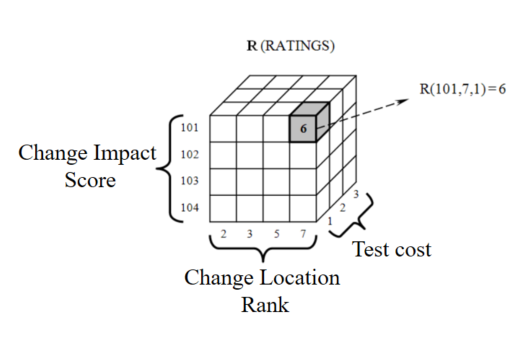
\includegraphics[width=0.75\linewidth]{./RM.png}
	\vspace*{3pt}
	\caption{An Example of Multidimensional Recommender System}
	\label{fig:rm}
\end{figure}


Figure ~\ref{fig:rm} shows an example of our recommender system.
Value $R$ in this figure indicates that, the ranking score for 
testing the class 101 of the system with location rank 7 and test
cost 1 is equal to 6. 


\subsection{Optimization}
%After obtaining the recommendation list form our recommender system,
%we calculate average percentage of fault detected to measure the efficiency of 
%our approach. 
The final phase of our recommender system include a optimization module 
which aimed for enhance the efficiency of the system.
To do this, we applied \textit{Genetic Algorithm} to suggest the best order of test
case for optimum results for different testing goals.
In this scenario we simulated different testing goals such as:
test the system with time constraint, testing the system to get maximum 
fault detection percentage, and testing the most frequently used components of the system. 
Initial population of our GA are the output list of our recommender system. 

%
%\begin{algorithmc}
%	\SetKwInOut{Input}{Input}
%	\SetKwInOut{Output}{Output}
%	
%	\underline{function Euclid} $(a,b)$\;
%	\Input{Two nonnegative integers $a$ and $b$}
%	\Output{$\gcd(a,b)$}
%	\eIf{$b=0$}
%	{
%		return $a$\;
%	}
%	{
%		return Euclid$(b,a\mod b)$\;
%	}
%	\caption{Euclid's algorithm for finding the greatest common divisor of two nonnegative integers}
%\end{algorithmc}


\subsubsection{Fitness Function}

We defined fitness function as direct proportional to 
the average relevance of a recommendation to the test goal. 

\subsubsection{Crossover}

\subsubsection{Mutation}





%\textbf{Step A:} Code metrics and change history collection:  
%In order to run our experiment we implemented a risk measurement tool.
%The tool has following feature:
%At the first step we used a commercial tool named Understand to extract code metrics.
%This tool provide code metrics in class and file level. 
%In our experiment we only used class level metrics. 
%Among 42 static code metrics which can be obtained from Understand 
%we only applied 8 of them in our experiment.  
%In second phase of our experiment design we collected change history be found
%metrics which can  in table ~\ref{tab:metrics}.\\
%\textbf{Step B:} Page rank calculation \\
%\textbf{Step C:} Calculate final risk score.\\ 
%
%
%
%\textbf{Step A: Code metrics and change history collection}\\
%Among 42 static code metric which Understand provided any many
%other change history metric we selected xx metric which can be found it 
%Table ~\ref{tab:metrics}. Feature selection can be overwhelming specially 
%if it is going to be heuristic, otherwise we calculate information gain ratio 
%to determine the most effective metrics among whole bunch of available metrics.
%The higher gain ratio determines that particular metric plays more significant
%to predict class labels than other metrics. 
%In this study we set out label as a boolean value which mean 
%1 indicates that in that class we observed at least one bug repost and 0 
%means no bug report yet.    be found in table ~\ref{tab:metrics}.\\
%
%\textbf{Step B: Page rank calculation}\\
%During the evaluation experiment we find out that effectives of each metric
%is slightly correlated to the context of object. 
%For example in DASCP we got higher gain ratio for Age of file than other two applications. 
%% short description about metrics and statics of it  
%In the next phase after selecting most correlated metric to the label 
%we applied multinomial regression model to calculate the weight of each
%metrics. 
%% short description about multinomial regression
%On the part of our experiment we performed multiple linear regression
%analysis to design a linear model for our dependant metric and 
%their relation to the buggy classes. \\
%In order to validate our classification model we applied 
%cross fold validation in our training data set. 
%For instance we have 200 classes that 50 of them at least have been reported a bug,
%choose 50 random classes for training set and then among that 50 random classes
%we mixed 10 of them with unlabled data and added 10 unlabled data into our training set
%then we repeat that process for several times later 
%we calculate accuracy by the following measures:
%
%
%\textbf{Step C: Final Risk Calculation.}\\
%In this step we aim to calculate the importance of risk location other than risk value itself. 
%We believe the location of change has a significant role in the riskiness rate. 
%We have got inspired form Huang [] research which claimed “Where the change takes place”. 
%But in their research they focused in the hot path of the source code such as loop or 
%primitive functions while in our research we are calculating the value of call graph for each class.\\ 
%There are two main reason why we need to consider call path besides code metrics and change history;
%first, those classes that has more connections with others are 
%more significant and they could be a base of other classes,
%specially (to avoid cascading regression we need to fix the source of leak!), other than that those 
%classed are more executed or called as a result they are 
%consume higher amount of CPU, RAM or other resources. 
%In order to calculate the call graph score for each 
%classes we used Understand tool to extract class dependency. 
%Understand provide three feature which are: References, From Entity and To Entities.
%
%%// more description about understand ---> paraf compeletly
%% Micro Interaction Metrics for Defect Prediction 
%We collected CMs at Time P as shown in Figure 2 since
%CMs can be extracted from a snapshot. We used the Understand tool [33] to extract CMs. The Understand tool
%extracts 24 file-level and 18 class-level metrics such as Chidamber and Kemerer [5] and Object-Oriented metrics. If
%a file has more than one class, we derived file-level metrics from multiple class-level metrics. The Understand tool
%mostly provides two kinds of metrics: Avg* and Count*. To
%generate file-level metrics from multiple classes in a file, we
%averaged Avg* class-level metrics. However, when we get
%file-level metrics from Count* classs-level metrics, we added
%the values together. We used all 42 CMs for our experiments.
%Selected CMs are listed in Table 3.
%
%
%%// in another paper they used worst case for call graph, ref shortly and why it is not related to my work
%
%
%The main idea of this algorithm is most important websites receive more links. 
%In our study we assumed each class as a web page and relationship between classes as hyper link.
%[] shows the formula of this algorithm:
%
%\fbox{\begin{minipage}{20em}
%		Final risk = Initial Risk * Pagerank score
%	\end{minipage}}
%	
%	
%	\textbf{Step C: Final risk score}
%	
%	We rely on static graph between classes with other error prone features of code. 
%	With those two metrics, we have a grid for assessing the criticality of any class in the system. 
%	Classes with high values in both metrics should be identified and reported to testers, 
%	as a residual error in those components will more likely deeply impact the whole system.
%	Concerning what we discussed above, we suggested this formula to calculate final risk score for each classes: CHRisk is the value of gained risk from step A, and Pagerank score is the call graph score from Step B. 
%	
%	\begin{algorithm}
%		\caption{Risk evaluation algorithm}
%		\label{CHalgorithm}
%		\begin{algorithmic}[1]
%			\State \textbf{Input:} \emph{Initiall risk list IR(), Pagerank score list PS()}
%			\State \textbf{Output:} \emph{Ranked list of Classes RC()}
%			\Procedure{Risk\textendash Evaluation}{}
%			\If {$i = \textit{0}$} 
%			%\state \emph{Update entire dataset}			
%			\While{$i\not=listLenght$}
%			\State $i \gets i + 0.1$ 
%			\EndWhile\label{euclidendwhile}
%			\EndIf		
%			\For{each node $i$ \Pisymbol{psy}{206} $IR$ }
%			\State $ \textit{FR(i)} \gets \textit{PS(i)} * \textit{IR(i)} $. 
%			\EndFor
%			\State $ \textit{RC} \gets \textit{Rank(C, FR)} $ 
%			\State \textbf{return} \emph{RC}
%			\EndProcedure
%		\end{algorithmic}
%	\end{algorithm}
%
%
